\documentclass[11pt,a4paper]{article}
\usepackage[margin=2.2cm]{geometry}
\usepackage{amsmath,amssymb,amsfonts}
\usepackage{booktabs,array,tabularx}
\usepackage{enumitem}
\usepackage{xcolor}
\usepackage{tikz}
\usetikzlibrary{arrows.meta,positioning,shapes.geometric}
\usepackage[colorlinks=true,linkcolor=blue!50!black,urlcolor=blue!50!black]{hyperref}
\usepackage{titlesec}
\titleformat{\section}{\large\bfseries}{\thesection}{0.8em}{}
\titleformat{\subsection}{\normalsize\bfseries}{\thesubsection}{0.8em}{}
\setlength{\parindent}{0pt}
\setlength{\parskip}{5pt}

\newcommand{\I}{\mathcal{I}}
\newcommand{\F}{\mathcal{F}}
\newcommand{\G}{\mathcal{G}}
\newcommand{\M}{\mathcal{M}}
\newcommand{\N}{\mathcal{N}}
\newcommand{\A}{\mathcal{A}}
\newcommand{\desc}[1]{\par\vspace{-2pt}{\small\color{black!75}\textit{Meaning:} #1}\par\vspace{4pt}}

\title{\textbf{EV Charging Network Optimisation}\\[3pt]
\large F2: continuous-time MILP\\[2pt]
\normalsize EV $\rightarrow$ charger (FCS / MCS) assignment + mobile charger routing}
\author{CP 320 OR for Mobility Management, course project}
\date{2 October 2026, revised 14 October 2026}

\begin{document}
\maketitle

\textbf{About this version.} The formulation does not depend on any particular dataset. An instance is just the list of inputs in Section~\ref{sec:data}: locations, energy demands, request times, station and van data, and a travel distance/time matrix. Any data source that provides these (synthetic, real, or a benchmark) can be used without changing the model. The earlier revision tied the inputs to the Solomon VRPTW instances; that link has been removed. Equation numbers are unchanged.

\textbf{Relation to F1.} F1 split the peak into time slots and let FCS charging start only at slot boundaries. F2 removes the slots: each EV has one continuous start time $S_i$, each FCS gun is a separate machine, and EVs on the same gun are ordered with either-or (disjunctive) constraints. F2 also adds energy cost, priority-weighted inconvenience and lateness to the objective.

%=====================================================================
\section{Problem}

During the evening peak $[0,T]$ a set of parked EVs raise charging requests. Each request must be served by exactly one resource: either the EV drives itself to a fixed charging station (FCS, 2 guns of 22\,kW each), or a mobile charging van (MCS) leaves the depot, drives to the EV, charges it (one EV at a time) and moves on, returning to the depot by $T$. We decide
\begin{enumerate}[leftmargin=1.6em,itemsep=1pt]
  \item which resource serves each EV (a gun of a station, or a van),
  \item the order in which each van visits its EVs and each gun charges its EVs,
  \item the time every charging session starts,
\end{enumerate}
so that total operating cost plus a penalty for customer inconvenience is minimal and every request is served.

%=====================================================================
\section{Assumptions}
\begin{enumerate}[leftmargin=1.6em,itemsep=1pt]
  \item \textbf{Static, continuous time.} All requests of the peak are known at time $0$; request $i$ becomes active at its request time $r_i$. All times are real numbers in $[0,T]$; there are no slots.
  \item An EV served by an FCS drives there itself (one way) on its own battery, waits for a free gun, and stays until charged. An EV can only use an FCS within its remaining range.
  \item An EV served by an MCS stays parked at its location; the van comes to it.
  \item Each FCS gun and each MCS charges one EV at a time, with no pre-emption, at constant power.
  \item A van's driving energy and delivered energy come from the same battery; there is no recharging of the van during the peak. Vans leave the depot at time $0$ (leaving later is equivalent to waiting at the first EV).
  \item Every request must be fully charged by $T$ (hard); finishing after the desired time $l_i$ is allowed but penalised (soft).
  \item Travel times are fixed (no congestion) and the same speed $v$ applies to every trip.
\end{enumerate}

%=====================================================================
\section{Instance data: what the model needs}\label{sec:data}

\subsection{Inputs (from the project brief)}
\begin{tabularx}{\textwidth}{@{}>{\raggedright\arraybackslash}p{3.0cm}>{\raggedright\arraybackslash}p{5.6cm}X@{}}
\toprule
\textbf{Entity} & \textbf{Input} & \textbf{Symbol} \\
\midrule
EV request $i$ & location; energy demand; request time; desired ready time; remaining range & node $i$; $E_i$ (kWh); $r_i$, $l_i$ (h); $R_i$ (km) \\
Fixed station $f$ & location; number of guns; power per gun & node $f$; $|\G_f|=2$; $P^F=22$\,kW \\
Mobile vans & depot location; battery; max EVs per period; charging power; driving consumption; efficiency; speed & node $0$; $B_m$; $Q_m$; $P^M$; $\beta$; $\eta$; $v$ \\
Road network & distance / travel time between key locations & $d_{if},t_{if}$; $d_{ij},t_{ij}$ (Section~\ref{sec:dist}) \\
Costs & per km, per van, per kWh, per hour & $c^{EV},c^M,c^F_m,\pi^F,\pi^M,c^W,c^L$ \\
Horizon & length of the evening peak & $T$ (h) \\
\bottomrule
\end{tabularx}

\subsection{Derived quantities (computed before solving)}
\begin{tabularx}{\textwidth}{@{}>{\raggedright\arraybackslash}p{5.0cm}X@{}}
\toprule
$\tau^F_i=E_i/P^F,\quad \tau^M_i=E_i/P^M$ & charging duration of EV $i$ at an FCS gun / by a van (h). The brief lists ``charging duration'' as an input; with constant power it follows from $E_i$. \\
$\F_i=\{f: d_{if}\le R_i\}$ & stations EV $i$ can reach on its remaining range \\
$w_i=1+\kappa\,(1-R_i/R_{\max})$ & priority weight ($\ge1$); EVs with little range left count more. $\kappa\ge0$ sets how strongly; $\kappa=0$ gives all EVs equal weight. Any other priority rule can be used instead. \\
$d,\ t$ matrices & see Section~\ref{sec:dist} \\
\bottomrule
\end{tabularx}

\subsection{Illustrative parameter values}
These are starting values for experiments, not part of the model; all are meant to be varied in the analysis.

\begin{tabularx}{\textwidth}{@{}l>{\raggedright\arraybackslash}p{4.6cm}X@{}}
\toprule
\textbf{Parameter} & \textbf{Value} & \textbf{Note} \\
\midrule
$T$ & 3--5 h & evening peak \\
$|\G_f|$, $P^F$ & 2 guns, 22\,kW & from the brief \\
$P^M$ & 30\,kW & van charger \\
$v$, $\beta$, $\eta$ & 25\,km/h, 0.25\,kWh/km, 0.9 & \\
$B_m$, $Q_m$, $|\M|$ & 150\,kWh, 6, 1--6 & \\
$E_i$, $R_i$ & 10--40\,kWh, 3--40\,km & $R_{\max}=40$, $\kappa=2$ \\
$c^{EV}$, $c^M$, $c^F_m$ & Rs\,4/km, Rs\,15/km, Rs\,1500 & van km includes driver time \\
$\pi^F$, $\pi^M$ & Rs\,8.7/kWh, Rs\,10.7/kWh & van energy = grid price + battery wear \\
$c^W$, $c^L$ & Rs\,200/h, Rs\,300/h & value of time; keep $c^L>c^W$ \\
\bottomrule
\end{tabularx}

%=====================================================================
\section{Distances, travel times and routes}\label{sec:dist}

\subsection{Which numbers the model needs}
The MILP never works on the street network itself. It works on a small \emph{complete graph of key locations}: the van depot, the $n$ EV locations and the FCS locations. It needs only
\begin{itemize}[leftmargin=1.4em,itemsep=1pt]
  \item $d_{if}, t_{if}$: EV $i$ $\to$ FCS $f$ (the EV's own trip),
  \item $d_{ij}, t_{ij}$: between the depot and EVs and between pairs of EVs (the van's trips).
\end{itemize}
Vans never visit an FCS and EVs never drive to each other, so FCS$\to$FCS and FCS$\to$EV entries are not needed. Each entry is the length (or time) of the \emph{shortest path} between the two locations, with $t=d/v$. They are computed \textbf{once, before optimisation}; they are parameters, not variables. The matrix may be asymmetric (one-way streets), because the model uses directed arcs.

\subsection{Two ways to obtain the matrix}
\begin{enumerate}[leftmargin=1.6em,itemsep=2pt]
  \item \textbf{From coordinates.} If only planar $(x,y)$ positions are available,
  $d_{ab}=\rho\sqrt{(x_a-x_b)^2+(y_a-y_b)^2}$, where $\rho\ge1$ is a detour factor for city roads (typically $1.2$--$1.4$; $\rho=1$ is pure straight-line). No shortest-path algorithm is needed.
  \item \textbf{From a road network.} On a road graph $G_R=(V_R,E_R)$ (e.g.\ OpenStreetMap), snap each key location to its nearest road node and run Dijkstra once from every key node (edge weight = length for $d$, length/speed for $t$), keeping only the values to other key nodes. Store the predecessor trees so the street path of any arc chosen by the MILP can be drawn afterwards.
\end{enumerate}

\subsection{How a van route is represented}
A route is a chain of arcs on the complete graph: $x_{ijm}=1$ means van $m$ goes from location $i$ straight to location $j$ (along the precomputed shortest path). Example: $x_{0,3,m}=x_{3,7,m}=x_{7,n+1,m}=1$ means depot $\to$ EV 3 $\to$ EV 7 $\to$ depot, with charging start times
\[
S_3=\max\{r_3,\;t_{03}\},\qquad S_7=\max\{r_7,\;S_3+\tau^M_3+t_{37}\},
\]
which is exactly what constraints \eqref{eq:release}, \eqref{eq:depart} and \eqref{eq:seq} enforce. Node $n+1$ is a copy of the depot, so a route starts at $0$ and ends at $n+1$.

\begin{center}
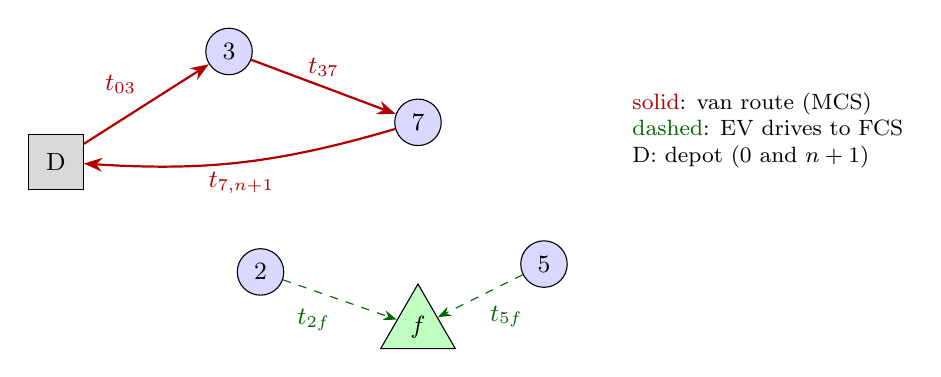
\begin{tikzpicture}[>=Stealth, every node/.style={font=\small}]
  \node[draw,fill=black!15,minimum size=7mm] (D) at (0,0) {D};
  \node[circle,draw,fill=blue!15] (e3) at (2.2,1.4) {3};
  \node[circle,draw,fill=blue!15] (e7) at (4.6,0.5) {7};
  \node[circle,draw,fill=blue!15] (e2) at (2.6,-1.4) {2};
  \node[circle,draw,fill=blue!15] (e5) at (6.2,-1.3) {5};
  \node[regular polygon,regular polygon sides=3,draw,fill=green!25,inner sep=1.5pt] (f1) at (4.6,-2.1) {$f$};
  \draw[->,thick,red!70!black] (D) -- node[above left]{$t_{03}$} (e3);
  \draw[->,thick,red!70!black] (e3) -- node[above]{$t_{37}$} (e7);
  \draw[->,thick,red!70!black] (e7) to[bend left=10] node[below]{$t_{7,n+1}$} (D);
  \draw[->,dashed,green!40!black] (e2) -- node[below left]{$t_{2f}$} (f1);
  \draw[->,dashed,green!40!black] (e5) -- node[below right]{$t_{5f}$} (f1);
  \node[anchor=west,align=left,font=\footnotesize] at (7.2,0.4) {
    \textcolor{red!70!black}{solid}: van route (MCS)\\
    \textcolor{green!40!black}{dashed}: EV drives to FCS\\
    D: depot ($0$ and $n+1$)};
\end{tikzpicture}
\end{center}

%=====================================================================
\section{Sets, parameters and decision variables}\label{sec:sets}

\subsection*{Sets}
\begin{tabularx}{\textwidth}{@{}lX@{}}
\toprule
$\I=\{1,\dots,n\}$ & EV charging requests \\
$\F$ & fixed charging stations (FCS) \\
$\G_f$ & guns (charging points) of FCS $f$, $|\G_f|=2$; $\G=\bigcup_{f}\G_f$, and $f(g)$ is the station of gun $g$ \\
$\F_i=\{f\in\F: d_{if}\le R_i\}$ & FCS that EV $i$ can reach on its remaining range \\
$\G_i=\bigcup_{f\in\F_i}\G_f$ & guns EV $i$ can use \\
$\M$ & mobile charging vans (MCS) \\
$0,\;n+1$ & depot as start node and as end node (same location) \\
$\N=\{0\}\cup\I\cup\{n+1\}$ & routing nodes \\
$\A=\{(i,j): i\in\{0\}\cup\I,\ j\in\I\cup\{n+1\},\ i\ne j,\ (i,j)\neq(0,n+1)\}$ & allowed van arcs \\
$\mathcal{P}_g=\{(i,j)\in\I^2: i<j,\ g\in\G_i\cap\G_j\}$ & pairs of EVs that could share gun $g$ \\
\bottomrule
\end{tabularx}

\subsection*{Parameters}
\begin{tabularx}{\textwidth}{@{}lX@{}}
\toprule
$E_i$ & energy demand of EV $i$ (kWh) \\
$r_i,\ l_i$ & request (release) time and desired completion time of EV $i$ (h), $0\le r_i\le l_i$ \\
$R_i$ & remaining driving range of EV $i$ (km) \\
$w_i\ge1$ & priority weight of EV $i$ \\
$P^F,\ P^M$ & charging power of an FCS gun (22\,kW) / of an MCS (kW) \\
$\tau^F_i=E_i/P^F,\ \tau^M_i=E_i/P^M$ & charging duration of EV $i$ at an FCS / by an MCS (h) \\
$d_{if},\ t_{if}$ & shortest-path distance (km) / travel time (h), EV $i\to$ FCS $f$ \\
$d_{ij},\ t_{ij}$ & shortest-path distance / travel time between routing nodes, $t_{ij}=d_{ij}/v$ \\
$v$ & travel speed (same for all trips) \\
$B_m$ & usable battery capacity of MCS $m$ (kWh) \\
$Q_m$ & maximum number of EVs MCS $m$ may serve in the period \\
$\beta$ & van driving consumption (kWh/km) \\
$\eta\in(0,1]$ & MCS charging efficiency (battery $\to$ EV) \\
$T$ & length of the planning period (h) \\
$c^{EV},\ c^{M}$ & cost per km of EV driving / van driving \\
$c^{F}_m$ & fixed dispatch cost of van $m$ (driver, depreciation) \\
$\pi^F,\ \pi^M$ & cost per kWh of grid energy at an FCS / of energy stored in a van battery \\
$c^W$ & inconvenience cost per hour of time lost by the driver \\
$c^L$ & lateness cost per hour beyond $l_i$ \\
$M^M_{ij}=T+\tau^M_i+t_{ij}$ & big-M for van sequencing \\
$M^F_i=T+\tau^F_i$ & big-M for gun sequencing \\
\bottomrule
\end{tabularx}

\subsection*{Decision variables}
\begin{tabularx}{\textwidth}{@{}llX@{}}
\toprule
$y_{ig}$ & $\in\{0,1\}$ & 1 if EV $i$ is charged at gun $g\in\G_i$ \\
$z_{im}$ & $\in\{0,1\}$ & 1 if EV $i$ is served by van $m$ \\
$x_{ijm}$ & $\in\{0,1\}$ & 1 if van $m$ drives arc $(i,j)\in\A$ \\
$u_m$ & $\in\{0,1\}$ & 1 if van $m$ is dispatched \\
$o_{ij}$ & $\in\{0,1\}$ & for $i<j$ sharing a gun: 1 if $i$ is charged before $j$ \\
$S_i$ & $\ge 0$ & time charging of EV $i$ starts (h), whichever resource \\
$L_i$ & $\ge 0$ & lateness of EV $i$ beyond $l_i$ (h) \\
\bottomrule
\end{tabularx}

\textbf{Short-hands} (linear expressions, not extra variables):
\[
Y_{if}=\sum_{g\in\G_f} y_{ig}\quad(\text{EV $i$ goes to FCS $f$}),\qquad
C_i = S_i + \tau^F_i\sum_{g\in\G_i} y_{ig} + \tau^M_i\sum_{m\in\M} z_{im}\quad(\text{completion time}).
\]
Because exactly one of the $y$/$z$ terms equals 1, $C_i$ is the start time plus the duration on the chosen resource.

%=====================================================================
\section{Objective}

\begin{align}
\min\ Z \;=\;& \underbrace{c^{EV}\sum_{i\in\I}\sum_{f\in\F_i} d_{if}\,Y_{if}}_{Z_1:\ \text{EV driving}}
\;+\; \underbrace{c^{M}\sum_{m\in\M}\sum_{(i,j)\in\A} d_{ij}\,x_{ijm}}_{Z_2:\ \text{van driving}}
\;+\; \underbrace{\sum_{m\in\M} c^{F}_m\,u_m}_{Z_3:\ \text{van dispatch}} \notag\\[2pt]
&+\; \underbrace{\pi^F\sum_{i\in\I}\sum_{g\in\G_i} E_i\,y_{ig} \;+\; \pi^M\sum_{i\in\I}\sum_{m\in\M}\frac{E_i}{\eta}\,z_{im}}_{Z_4:\ \text{energy}}
\;+\; \underbrace{c^W\sum_{i\in\I} w_i\,(C_i - r_i)}_{Z_5:\ \text{inconvenience}}
\;+\; \underbrace{c^L\sum_{i\in\I} w_i\,L_i}_{Z_6:\ \text{lateness}} \label{eq:obj}
\end{align}

\begin{description}[leftmargin=1.2em,itemsep=2pt,font=\normalfont\bfseries]
  \item[$Z_1$ EV driving.] Distance each FCS user drives to its station. It pushes EVs towards the \emph{nearest} FCS with a free gun: a closer station is cheaper, and a closer station also starts charging earlier, which lowers $Z_5$.
  \item[$Z_2$ van driving.] Total km of all van routes (fuel/wear/driver time per km).
  \item[$Z_3$ dispatch.] Fixed cost of every van that leaves the depot; with $Z_2$ this is the ``operating cost of MCS'' in the brief.
  \item[$Z_4$ energy.] The same kWh costs different amounts by resource: grid price at an FCS, versus van energy which is dearer per kWh and loses $1-\eta$ in transfer. This is the main reason an MCS is not used for everyone.
  \item[$Z_5$ inconvenience.] $C_i-r_i$ is the time from request until the car is fully charged: for an FCS user it is driving + queueing at the gun + charging; for an MCS user it is waiting for the van + charging. Multiplying by $w_i$ gives \emph{priority}: urgent EVs cost more per hour of delay, so the model serves them first. ($c^W\sum_i w_i r_i$ is a constant and can be dropped when solving.)
  \item[$Z_6$ lateness.] Penalty for finishing after the driver's desired time $l_i$, also priority-weighted.
\end{description}
All terms are in currency units; the weights $c^W,c^L$ convert time into money and can be varied to trade cost against service. $Z_1$--$Z_4$ are the operator's cost (the brief's main KPI) and should be reported separately from $Z_5$--$Z_6$.

%=====================================================================
\section{Constraints}

\subsection{Assignment}
\begin{equation}
\sum_{g\in\G_i} y_{ig} + \sum_{m\in\M} z_{im} = 1 \qquad \forall i\in\I \label{eq:assign}
\end{equation}
\desc{Every request is served by exactly one resource: one gun of one reachable FCS, or one van. If EV $i$ reaches no FCS ($\G_i=\emptyset$) it is forced onto a van, which is how range-critical EVs are protected.}

\subsection{Fixed charging stations (continuous time)}
\begin{equation}
S_i \;\ge\; r_i + \sum_{f\in\F_i} t_{if}\,Y_{if} \qquad \forall i\in\I \label{eq:fcsarr}
\end{equation}
\desc{An FCS user cannot start before it has been requested and has driven to its station. For an MCS user the sum is zero and this becomes $S_i\ge r_i$.}

\begin{align}
S_j &\ge S_i + \tau^F_i - M^F_i\,(3 - y_{ig} - y_{jg} - o_{ij}) && \forall g\in\G,\ (i,j)\in\mathcal{P}_g \label{eq:disj1}\\
S_i &\ge S_j + \tau^F_j - M^F_j\,(2 - y_{ig} - y_{jg} + o_{ij}) && \forall g\in\G,\ (i,j)\in\mathcal{P}_g \label{eq:disj2}
\end{align}
\desc{No two EVs overlap on the same gun. If both $i$ and $j$ use gun $g$ ($y_{ig}=y_{jg}=1$), then either $o_{ij}=1$ and \eqref{eq:disj1} forces $j$ to start after $i$ has finished, or $o_{ij}=0$ and \eqref{eq:disj2} forces the reverse. If either is not on $g$ the big-M switches both constraints off. With two guns per station this is exactly ``at most 2 EVs charging at an FCS at any moment'', without any time grid. $M^F_i=T+\tau^F_i$ is enough because $0\le S_i\le T$.}

\begin{equation}
\sum_{i\in\I}\tau^F_i\,y_{ig} \;\le\; T - \min_{i:\,g\in\G_i}\,(r_i+t_{i f(g)}) \qquad \forall g\in\G \label{eq:gunload}
\end{equation}
\desc{Valid inequality (implied by the others, added to tighten the LP relaxation): the total charging time on one gun cannot exceed the time it is available. It also gives a cheap aggregate capacity model if the instance is too large for the sequencing constraints.}

\begin{equation}
\sum_{i\in\I} y_{i g_1} \;\ge\; \sum_{i\in\I} y_{i g_2} \qquad \forall f\in\F,\ \G_f=\{g_1,g_2\} \label{eq:gunsym}
\end{equation}
\desc{Symmetry breaking: the two guns of a station are identical, so let gun 1 carry at least as many EVs as gun 2. Optional; it removes mirror solutions and speeds up branch-and-bound.}

\subsection{MCS routing}
\begin{align}
\sum_{j:(0,j)\in\A} x_{0jm} &= u_m && \forall m\in\M \label{eq:out}\\
\sum_{i:(i,n+1)\in\A} x_{i,n+1,m} &= u_m && \forall m\in\M \label{eq:in}\\
\sum_{i:(i,j)\in\A} x_{ijm} &= z_{jm} && \forall j\in\I,\ m\in\M \label{eq:flowin}\\
\sum_{k:(j,k)\in\A} x_{jkm} &= z_{jm} && \forall j\in\I,\ m\in\M \label{eq:flowout}
\end{align}
\desc{\eqref{eq:out}--\eqref{eq:in}: a dispatched van leaves the depot once and returns once; an unused van does neither. \eqref{eq:flowin}--\eqref{eq:flowout}: every EV assigned to van $m$ is entered once and left once by that van, i.e.\ visited exactly once; EVs not on $m$ are not touched by it. Together they make each van's arcs one path $0\to\dots\to n+1$ (plus possible cycles, removed by \eqref{eq:seq}).}

\subsection{MCS capacity and battery}
\begin{align}
\sum_{i\in\I} z_{im} &\le Q_m\,u_m && \forall m\in\M \label{eq:cap}\\
\sum_{i\in\I}\frac{E_i}{\eta}\,z_{im} + \beta\sum_{(i,j)\in\A} d_{ij}\,x_{ijm} &\le B_m\,u_m && \forall m\in\M \label{eq:batt}
\end{align}
\desc{\eqref{eq:cap}: a van serves at most $Q_m$ EVs, and none if it is not dispatched. \eqref{eq:batt}: the energy drawn from the van battery (energy delivered, grossed up for transfer losses, plus the energy to drive the whole route) must fit in its usable capacity.}

\subsection{MCS timing (one EV at a time, no subtours)}
\begin{align}
S_j &\ge t_{0j}\,x_{0jm} && \forall j\in\I,\ m\in\M \label{eq:depart}\\
S_j &\ge S_i + \tau^M_i + t_{ij} - M^M_{ij}\,(1-x_{ijm}) && \forall i,j\in\I,\ i\ne j,\ m\in\M \label{eq:seq}\\
S_i + \tau^M_i + t_{i,n+1} &\le T + (\tau^M_i + t_{i,n+1})\,(1-x_{i,n+1,m}) && \forall i\in\I,\ m\in\M \label{eq:return}
\end{align}
\desc{\eqref{eq:depart}: the first EV on a route cannot be started before the van (leaving at $0$) has driven to it. \eqref{eq:seq}: if van $m$ goes from $i$ to $j$, it must finish charging $i$ and drive to $j$ before starting $j$. This both prevents a van from charging two EVs at once and, because $\tau^M_i+t_{ij}>0$, makes start times strictly increase along a route so no cycle can close (MTZ-type subtour elimination). \eqref{eq:return}: the van is back at the depot by $T$.}

\subsection{Time windows and lateness}
\begin{align}
S_i &\ge r_i && \forall i\in\I \label{eq:release}\\
C_i &\le T && \forall i\in\I \label{eq:horizon}\\
L_i &\ge C_i - l_i && \forall i\in\I \label{eq:late}
\end{align}
\desc{\eqref{eq:release}: no charging before the request (a van that arrives early waits). It is implied by \eqref{eq:fcsarr} and kept for readability. \eqref{eq:horizon}: every EV is fully charged within the peak, which guarantees ``all requests satisfied''. \eqref{eq:late}: with $L_i\ge0$ and $L_i$ minimised in $Z_6$, $L_i=\max\{0,C_i-l_i\}$.}

\subsection{Van symmetry and domains}
\begin{align}
u_m &\ge u_{m+1} && m=1,\dots,|\M|-1 \label{eq:vansym}\\
y_{ig},\,z_{im},\,x_{ijm},\,u_m,\,o_{ij} &\in\{0,1\},\qquad S_i,\,L_i\ge 0 \label{eq:dom}
\end{align}
\desc{\eqref{eq:vansym}: vans are identical, so use them in index order (van 2 only if van 1 is used, etc.). \eqref{eq:dom}: variable domains.}

%=====================================================================
\section{The complete model}\label{sec:full}

With $Y_{if}=\sum_{g\in\G_f}y_{ig}$ and $C_i=S_i+\tau^F_i\sum_{g\in\G_i}y_{ig}+\tau^M_i\sum_{m}z_{im}$:

{\small
\begin{align*}
\min\quad & c^{EV}\sum_{i}\sum_{f\in\F_i} d_{if}Y_{if}+c^{M}\sum_{m}\sum_{(i,j)\in\A} d_{ij}x_{ijm}+\sum_{m} c^{F}_mu_m \\
&+\pi^F\sum_{i}\sum_{g\in\G_i} E_iy_{ig}+\pi^M\sum_{i}\sum_{m}\tfrac{E_i}{\eta}z_{im}
+c^W\sum_{i} w_i(C_i - r_i)+c^L\sum_{i} w_iL_i \tag{\ref{eq:obj}}\\[4pt]
\text{s.t.}\quad
& \textstyle\sum_{g\in\G_i} y_{ig} + \sum_{m} z_{im} = 1 && \forall i \tag{\ref{eq:assign}}\\
& S_i \ge r_i + \textstyle\sum_{f\in\F_i} t_{if}Y_{if} && \forall i \tag{\ref{eq:fcsarr}}\\
& S_j \ge S_i + \tau^F_i - M^F_i(3 - y_{ig} - y_{jg} - o_{ij}) && \forall g,\ (i,j)\in\mathcal{P}_g \tag{\ref{eq:disj1}}\\
& S_i \ge S_j + \tau^F_j - M^F_j(2 - y_{ig} - y_{jg} + o_{ij}) && \forall g,\ (i,j)\in\mathcal{P}_g \tag{\ref{eq:disj2}}\\
& \textstyle\sum_{i}\tau^F_iy_{ig} \le T - \min_{i:g\in\G_i}(r_i+t_{if(g)}) && \forall g \tag{\ref{eq:gunload}}\\
& \textstyle\sum_{i} y_{ig_1} \ge \sum_{i} y_{ig_2} && \forall f,\ \G_f=\{g_1,g_2\} \tag{\ref{eq:gunsym}}\\
& \textstyle\sum_{j} x_{0jm} = u_m,\quad \sum_{i} x_{i,n+1,m} = u_m && \forall m \tag{\ref{eq:out}, \ref{eq:in}}\\
& \textstyle\sum_{i} x_{ijm} = z_{jm},\quad \sum_{k} x_{jkm} = z_{jm} && \forall j\in\I,\ m \tag{\ref{eq:flowin}, \ref{eq:flowout}}\\
& \textstyle\sum_{i} z_{im} \le Q_mu_m && \forall m \tag{\ref{eq:cap}}\\
& \textstyle\sum_{i}\frac{E_i}{\eta}z_{im} + \beta\sum_{(i,j)\in\A} d_{ij}x_{ijm} \le B_mu_m && \forall m \tag{\ref{eq:batt}}\\
& S_j \ge t_{0j}x_{0jm} && \forall j\in\I,\ m \tag{\ref{eq:depart}}\\
& S_j \ge S_i + \tau^M_i + t_{ij} - M^M_{ij}(1-x_{ijm}) && \forall i\ne j\in\I,\ m \tag{\ref{eq:seq}}\\
& S_i + \tau^M_i + t_{i,n+1} \le T + (\tau^M_i + t_{i,n+1})(1-x_{i,n+1,m}) && \forall i,\ m \tag{\ref{eq:return}}\\
& S_i \ge r_i,\quad C_i \le T,\quad L_i \ge C_i - l_i && \forall i \tag{\ref{eq:release}--\ref{eq:late}}\\
& u_m \ge u_{m+1} && m<|\M| \tag{\ref{eq:vansym}}\\
& y,z,x,u,o\in\{0,1\},\quad S,L\ge 0 \tag{\ref{eq:dom}}
\end{align*}
}
Constraints \eqref{eq:gunload}, \eqref{eq:gunsym}, \eqref{eq:release} and \eqref{eq:vansym} are optional: they do not change the optimal value but help the solver or the reader.

%=====================================================================
\section{Model size and remarks}

\begin{tabularx}{\textwidth}{@{}lX@{}}
\toprule
Binaries & $\sum_i|\G_i| + n|\M| + |\A||\M| + |\M| + |\bigcup_g\mathcal{P}_g|$ (one $o_{ij}$ per pair). For $n=25$, $|\F|=5$, $|\M|=3$, every station reachable: $250+75+1{,}950+3+300\approx 2{,}600$. \\
Continuous & $2n$ ($S_i$, $L_i$). \\
Largest blocks & \eqref{eq:seq} with $n^2|\M|$ rows and \eqref{eq:disj1}--\eqref{eq:disj2} with $2\sum_g|\mathcal{P}_g|$ rows. \\
\bottomrule
\end{tabularx}

\begin{itemize}[leftmargin=1.4em,itemsep=2pt]
  \item \textbf{Solving.} Instances with $n\le 25$--$50$ are realistic for Gurobi/CPLEX directly. For larger $n$, shrink $\mathcal{P}_g$ (drop pairs whose request windows cannot overlap on $g$), restrict $\F_i$ to the $k$ nearest stations, or use \eqref{eq:gunload} alone in place of \eqref{eq:disj1}--\eqref{eq:disj2} as a capacity-only relaxation; these are also natural baselines for the RL / heuristic comparison.
  \item \textbf{Big-M values} are the smallest safe ones: $M^F_i=T+\tau^F_i$ since $0\le S_i,S_j\le T$ (plain $T$ is not safe when $i$ is on a faster van); $M^M_{ij}=T+\tau^M_i+t_{ij}$.
  \item \textbf{Infeasibility} means the fleet cannot serve everyone by $T$ (too few vans or guns, or vans' batteries too small). For experiments, add an ``unserved'' binary $s_i$ to \eqref{eq:assign} ($\dots+s_i=1$) with a large penalty in $Z$ and report how many EVs are unserved; in the analysis, report the smallest $|\M|$ or $T$ that makes an instance feasible.
  \item \textbf{Earliest start is optimal for a fixed plan.} Once the assignment and the order on every gun and van are fixed, starting every session as early as the constraints allow is optimal, because every time-dependent term in $Z$ grows with $C_i$. This is useful for heuristics and for RL, which then only need to choose assignments and orders.
  \item \textbf{Extensions (optional challenge).} Dynamic requests: re-solve this model on a rolling horizon with fixed past decisions. Time-varying prices: split $\pi^F$ by price period and charge $E_i$ at the price of the period(s) the session covers (see F3, scenarios S2 and S4). Congestion: time-dependent $t_{ij}$.
\end{itemize}

\end{document}
